
\chapter*{Prelude}

\vspace{-30pt}

Trigonometric identities are often presented as a big list of rules. 

\noindent\includegraphics[width=\linewidth]{assets/prelude/trig-identities.pdf}


\noindent Students are often asked to solve problems by applying a subset of those rules, \eg, $sin(0 - \theta) = -sin(\theta)$.

\begin{figure*}[h]
    \centering
    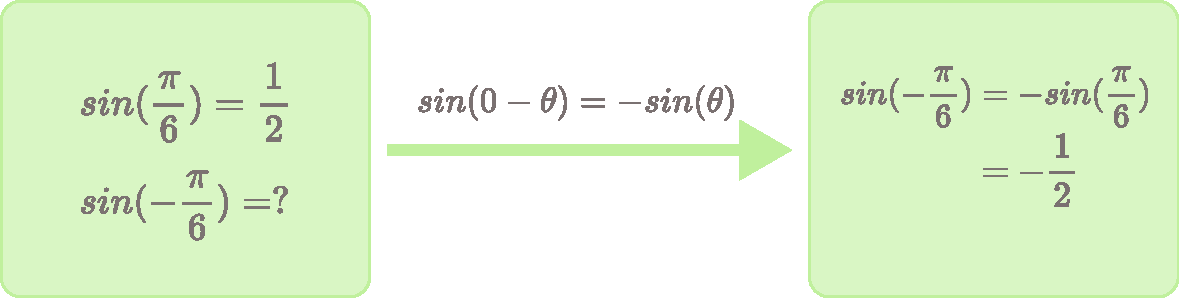
\includegraphics[width=0.75\linewidth]{assets/prelude/symbolic-transform.pdf}
    % \vspace{-10pt}
\end{figure*}

\setlength{\columnsep}{1em}
\setlength{\intextsep}{0em}
\begin{wrapfigure}{r}{.23\textwidth}
\vspace{-10pt}
  \begin{center}
    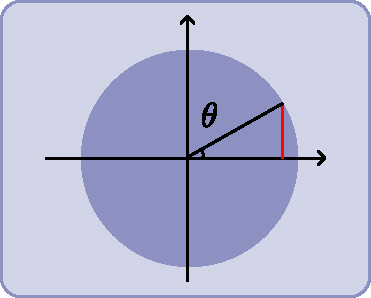
\includegraphics[width=0.23\textwidth]{assets/prelude/unit-circle.pdf}
  \end{center}
\end{wrapfigure}

A useful visual representation of this concept is the unit circle: on a Cartesian plane with a circle of radius $1$ centered at the origin, concrete values of trig functions are represented visually and rules are implicitly encoded as geometric transformations. For instance, the value of $sin(\theta)$ is the y-coordinate of a point on the circle, where the ray from the origin to the point forms angle $\theta$ with the x-axis.

To derive the identity rule visually, one only needs to note that $-\theta$ is a reflection about the x-axis, and observe that the y-coordinate is now a negative number. Instead of having to memorize a big set of rules, one can reduce this problem to a simple operation on the visual representation of a unit circle.

\vspace{10pt}
\begin{figure*}[h]
    \centering
    \includegraphics[width=0.70\linewidth]{assets/prelude/visual-transform.pdf}
    % \vspace{-10pt}
\end{figure*}

By translating the symbols to a visual representation, a unit circle, a student completely bypasses the tedious memorization of trig identities. While this is a much more retainable and robust representation for students, are we teaching representations like this to students? What does it take for students to internalize it? 
